%============================================================================
%  3D CFD Conjugate Heat-Transfer Model of a Prismatic HTGR Unit Cell
%  Interview deck for Radiant Nuclear — STAR format
%  Compile: pdflatex -> pdflatex   (run twice for TOC/refs)
%============================================================================
\documentclass[aspectratio=169,11pt]{beamer}

\usepackage[T1]{fontenc}
\usepackage{helvet}
\renewcommand\familydefault{\sfdefault}
\usepackage{sfmath}          % sans-serif math to match
\usepackage{amsmath}
\usepackage{graphicx}
\usepackage{booktabs}
\usepackage{colortbl}   % \rowcolor, \arrayrulecolor
\usepackage{array}
\usepackage{tikz}
\usepackage{pifont}
\usetikzlibrary{positioning,backgrounds,calc,shapes.geometric,arrows.meta,patterns}

% --- icon shims (map fontawesome names to pifont/dingbats) ---------------
\newcommand{\faCircle}{\ding{108}}
\newcommand{\faAngleRight}{\ding{228}}
\newcommand{\faCheckCircle}{\ding{51}}
\newcommand{\faExclamationTriangle}{\ding{115}}
\newcommand{\faBalanceScale}{\ding{47}}
\newcommand{\faArrowRight}{\ding{228}}
\newcommand{\faCube}{\ding{110}}
\newcommand{\faThLarge}{\ding{110}}

%----------------------------------------------------------------------------
%  RADIANT palette
%----------------------------------------------------------------------------
\definecolor{RadNavy}{HTML}{0B1E3F}   % deep base
\definecolor{RadNavy2}{HTML}{112A55}  % lighter navy
\definecolor{RadBlue}{HTML}{2E7DE0}   % electric primary
\definecolor{RadBlueL}{HTML}{6FA8EE}
\definecolor{RadAmber}{HTML}{F5A623}  % warm thermal accent
\definecolor{RadHot}{HTML}{E4572E}    % peak / limit (hot)
\definecolor{RadTeal}{HTML}{17A2B8}   % coolant
\definecolor{RadInk}{HTML}{16233A}    % body text
\definecolor{RadGray}{HTML}{5A6B85}   % muted
\definecolor{RadPanel}{HTML}{EEF3FB}  % light panel
\definecolor{RadPanel2}{HTML}{E2ECFA}
\definecolor{RadLine}{HTML}{CBD8EC}

%----------------------------------------------------------------------------
%  Beamer theme setup (custom, minimal)
%----------------------------------------------------------------------------
\usetheme{default}
\usecolortheme{default}
\setbeamertemplate{navigation symbols}{}
\setbeamercolor{normal text}{fg=RadInk}
\setbeamercolor{structure}{fg=RadBlue}
\setbeamercolor{itemize item}{fg=RadAmber}
\setbeamercolor{itemize subitem}{fg=RadBlue}
\setbeamercolor{block title}{fg=white,bg=RadNavy}
\setbeamercolor{block body}{fg=RadInk,bg=RadPanel}
\setbeamerfont{block title}{series=\bfseries}
\setbeamerfont{frametitle}{series=\bfseries}
\setbeamertemplate{itemize item}{\footnotesize\raisebox{0.15ex}{\color{RadAmber}\ding{108}}}
\setbeamertemplate{itemize subitem}{\footnotesize\color{RadBlue}\ding{228}}

% ---- custom frame title: accent bar + amber underline -------------------
\setbeamertemplate{frametitle}{%
  \nointerlineskip
  \begin{beamercolorbox}[wd=\paperwidth,ht=3.2ex,dp=1.4ex,leftskip=0.9cm,rightskip=0.4cm]{}%
    \tikz[baseline]{\node[anchor=base]{};}%
    \hspace*{-0.55cm}\raisebox{-0.15ex}{\tikz{\fill[RadAmber] (0,0) rectangle (0.13,1.9ex);}}\hspace{0.30cm}%
    {\color{RadNavy}\bfseries\large\insertframetitle}%
  \end{beamercolorbox}%
  \vspace{-0.2ex}\hspace*{0.9cm}{\color{RadLine}\rule{\dimexpr\paperwidth-1.3cm}{0.9pt}}%
  \vspace{0.4ex}
}

% ---- footer -------------------------------------------------------------
\setbeamertemplate{footline}{%
  \hbox{%
    \begin{beamercolorbox}[wd=\paperwidth,ht=2.6ex,dp=1.1ex]{}%
      \hspace{0.9cm}{\color{RadGray}\footnotesize Prismatic Microreactor Thermal Study \;\textbullet\; 3D CFD}%
      \hfill{\color{RadGray}\footnotesize Radiant Nuclear \;\textbullet\; \insertframenumber}\hspace{0.7cm}%
    \end{beamercolorbox}%
  }\vspace{1.2ex}%
}

%----------------------------------------------------------------------------
%  Helper commands
%----------------------------------------------------------------------------
% rounded stat tile
\newcommand{\stattile}[4]{% color, big number, unit/sub, label
  \begin{tikzpicture}
    \node[rounded corners=6pt, fill=#1, text=white, inner sep=7pt,
          minimum width=3.05cm, minimum height=1.75cm, align=center] {
      {\bfseries\large #2}\,{\small #3}\\[1pt]{\scriptsize #4}
    };
  \end{tikzpicture}}

% STAR chip
\newcommand{\starchip}[3]{% letter, word, color
  \begin{tikzpicture}
    \node[circle, fill=#3, text=white, minimum size=0.72cm, inner sep=0pt,
          font=\bfseries]{#1};
  \end{tikzpicture}%
  \;{\color{RadNavy}\bfseries #2}}

\newcommand{\kw}[1]{{\color{RadBlue}\bfseries #1}}
\newcommand{\amberkw}[1]{{\color{RadHot}\bfseries #1}}

% table rules
\setlength{\arrayrulewidth}{0.5pt}
\arrayrulecolor{RadLine}
\renewcommand{\arraystretch}{1.25}

%----------------------------------------------------------------------------
%  SECTION DIVIDER frame
%----------------------------------------------------------------------------
\newcommand{\sectiondivider}[4]{% letter, WORD, subtitle, number
\begin{frame}[plain]
\begin{tikzpicture}[remember picture,overlay]
  \fill[RadNavy] (current page.south west) rectangle (current page.north east);
  % thermal gradient strip on right
  \shade[left color=RadNavy, right color=RadHot]
     ([xshift=-2.6cm]current page.north east) rectangle (current page.south east);
  \fill[RadNavy,opacity=0.55] ([xshift=-2.6cm]current page.north east) rectangle (current page.south east);
  % big ghost letter
  \node[anchor=east, text=RadNavy2, font=\fontsize{190}{190}\bfseries,opacity=0.9]
        at ([xshift=-0.2cm,yshift=-0.2cm]current page.east) {#1};
  % stage label
  \node[anchor=west, text=RadAmber, font=\bfseries\Large] at ([xshift=1.3cm,yshift=1.75cm]current page.west) {\ STAGE #4};
  \node[anchor=west] at ([xshift=1.25cm,yshift=0.45cm]current page.west)
        {\color{white}\fontsize{40}{44}\selectfont\bfseries #2};
  \fill[RadAmber] ([xshift=1.35cm,yshift=-0.45cm]current page.west) rectangle ([xshift=3.15cm,yshift=-0.35cm]current page.west);
  \node[anchor=north west, text=RadBlueL, font=\large] at ([xshift=1.35cm,yshift=-0.85cm]current page.west)
        {\begin{minipage}{8.7cm}#3\end{minipage}};
\end{tikzpicture}
\end{frame}}

%============================================================================
\begin{document}

%----------------------------------------------------------------------------
%  TITLE
%----------------------------------------------------------------------------
\begin{frame}[plain]
\begin{tikzpicture}[remember picture,overlay]
  \fill[RadNavy] (current page.south west) rectangle (current page.north east);
  % subtle hex motif top-right
  \foreach \i in {0,1,2}{
    \node[regular polygon, regular polygon sides=6, draw=RadNavy2, line width=1.2pt,
          minimum size=2.6cm+\i*1.3cm, rotate=30] at ([xshift=-1.6cm,yshift=-1.4cm]current page.north east){};
  }
  % thermal gradient bar
  \shade[bottom color=RadBlue, top color=RadHot]
     ([xshift=1.25cm,yshift=1.15cm]current page.west) rectangle ([xshift=1.42cm,yshift=3.9cm]current page.west);
  % eyebrow
  \node[anchor=west, text=RadAmber, font=\bfseries\small] at ([xshift=1.75cm,yshift=3.5cm]current page.west)
        {RADIANT NUCLEAR \;\textbullet\; THERMAL MODELING INTERVIEW};
  % title
  \node[anchor=north west] at ([xshift=1.7cm,yshift=3.15cm]current page.west)
    {\begin{minipage}{13.4cm}
       \color{white}\fontsize{22}{27}\selectfont\bfseries
       3D CFD Conjugate Heat-Transfer Model of a Prismatic HTGR Unit Cell
     \end{minipage}};
  \node[anchor=north west] at ([xshift=1.75cm,yshift=-0.25cm]current page.west)
    {\begin{minipage}{12.2cm}\color{RadBlueL}\large
       Predicting peak TRISO fuel temperature under normal operation --- and proving the number is trustworthy.
     \end{minipage}};
  % bottom meta band
  \fill[RadNavy2] (current page.south west) rectangle ([yshift=1.35cm]current page.south east);
  \node[anchor=west, text=white] at ([xshift=1.7cm,yshift=0.68cm]current page.south west)
        {\footnotesize\bfseries Samay Shah};
  \node[anchor=west, text=RadBlueL] at ([xshift=1.7cm,yshift=0.30cm]current page.south west)
        {\footnotesize\ Helium-cooled microreactor (Kaleidos class) \;\textbullet\; OpenFOAM~7 CHT};
  \node[anchor=east, text=RadAmber] at ([xshift=-1.4cm,yshift=0.5cm]current page.south east)
        {\footnotesize\bfseries STAR walkthrough};
\end{tikzpicture}
\end{frame}

%----------------------------------------------------------------------------
%  ROADMAP (STAR)
%----------------------------------------------------------------------------
\begin{frame}{How I'll walk through this}
\vspace{0.1cm}
{\color{RadGray}\small A single engineering story, told in four moves.}
\vspace{0.3cm}

\begin{columns}[T]
\begin{column}{0.5\textwidth}
\setbeamercolor{block body}{bg=RadPanel}
\begin{block}{\starchip{S}{Situation}{RadBlue}}
\footnotesize One number decides everything: does the TRISO fuel stay under \amberkw{1600\,\textdegree C}? Peak fuel temperature is the licensing-relevant quantity.
\end{block}
\begin{block}{\starchip{A}{Action}{RadAmber}}
\footnotesize A 3D conjugate heat-transfer model in OpenFOAM --- unit-cell geometry, two coupled regions, an embedded fuel source, and a decisive \kw{mesh-quality fix}.
\end{block}
\end{column}
\begin{column}{0.5\textwidth}
\begin{block}{\starchip{T}{Task}{RadTeal}}
\footnotesize The take-home: build a \kw{3D CFD} model predicting peak fuel temperature (normal operation) --- and \kw{demonstrate validation}, not just plot a field.
\end{block}
\begin{block}{\starchip{R}{Result}{RadHot}}
\footnotesize \amberkw{670 $\pm$ 2\,\textdegree C}, grid-independent, corroborated three ways. $\sim$930\,\textdegree C of margin to the 1600\,\textdegree C limit.
\end{block}
\end{column}
\end{columns}
\end{frame}

%============================================================================
\sectiondivider{S}{SITUATION}{The safety question that defines this reactor class --- and the single number that answers it.}{01}

%----------------------------------------------------------------------------
\begin{frame}{The safety case rests on peak fuel temperature}
\begin{columns}[T]
\begin{column}{0.57\textwidth}
\begin{itemize}\small
  \item Radiant's Kaleidos class is a \kw{helium-cooled, TRISO-fueled} microreactor in a prismatic graphite block.
  \item \kw{TRISO fuel} = fissile kernels in ceramic layers that retain fission products up to $\sim$\amberkw{1600\,\textdegree C}.
  \item Stay below that limit and the reactor is \kw{safe by design} --- so the whole thermal case reduces to one question.
\end{itemize}
\vspace{0.1cm}
\begin{block}{The governing question}
\small Does the fuel stay below \amberkw{1600\,\textdegree C} at full power --- and how much \kw{margin} is there?
\end{block}
\vspace{0.05cm}
{\color{RadGray}\footnotesize A prediction is only useful with evidence it is correct.}
\end{column}
\begin{column}{0.43\textwidth}
\centering
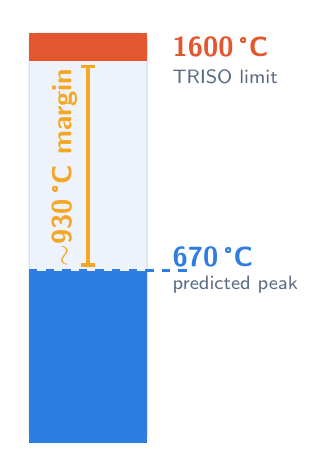
\begin{tikzpicture}[font=\scriptsize]
  % thermometer-style margin bar
  \def\H{5.2}
  \draw[rounded corners=3pt, fill=RadPanel, draw=RadLine] (0,0) rectangle (1.5,\H);
  % limit
  \fill[RadHot] (0,\H-0.35) rectangle (1.5,\H);
  \node[anchor=west, text=RadHot, font=\bfseries] at (1.7,\H-0.17) {1600\,\textdegree C};
  \node[anchor=west, text=RadGray] at (1.7,\H-0.55) {TRISO limit};
  % operating peak at ~670/1600 of height
  \pgfmathsetmacro\pk{\H*0.42}
  \fill[RadBlue] (0,0) rectangle (1.5,\pk);
  \draw[RadBlue,dashed,line width=1pt] (0,\pk) -- (2.0,\pk);
  \node[anchor=west, text=RadBlue, font=\bfseries] at (1.7,\pk+0.18) {670\,\textdegree C};
  \node[anchor=west, text=RadGray] at (1.7,\pk-0.18) {predicted peak};
  % margin brace
  \draw[RadAmber, line width=1.4pt, {|[width=5pt]}-{|[width=5pt]}] (0.75,\pk+0.05) -- (0.75,\H-0.4);
  \node[text=RadAmber, font=\bfseries, rotate=90] at (0.45,{(\pk+\H-0.4)/2}) {$\sim$930\,\textdegree C margin};
\end{tikzpicture}\\[2pt]
{\color{RadGray}\scriptsize Normal-operation headline result (this study).}
\end{column}
\end{columns}
\end{frame}

%============================================================================
\sectiondivider{T}{TASK}{Turn that question into a well-posed, validated 3D CFD problem I could actually run and defend.}{02}

%----------------------------------------------------------------------------
\begin{frame}{The take-home, and how I scoped it}
\begin{columns}[T]
\begin{column}{0.5\textwidth}
\begin{block}{What was asked}
\small Build a \kw{3D CFD} model to predict peak fuel temperature, and \kw{demonstrate validation} --- for the normal-operation scenario.
\end{block}
\vspace{0.1cm}
\textbf{\color{RadNavy}Scoping decisions}
\begin{itemize}\footnotesize
  \item \kw{Representative unit cell}, not a whole block --- standard prismatic-HTGR practice; tractable mesh, clean to validate.
  \item \kw{Steady state} --- only the equilibrium peak matters; transient-to-steady is infeasible (fluid CFL $\sim$10$^{-4}$\,s vs.\ minutes).
  \item Unit-cell \kw{symmetry} $\Rightarrow$ adiabatic walls $\Rightarrow$ an \emph{exact} energy balance.
\end{itemize}
\end{column}
\begin{column}{0.5\textwidth}
\vspace{0.2cm}
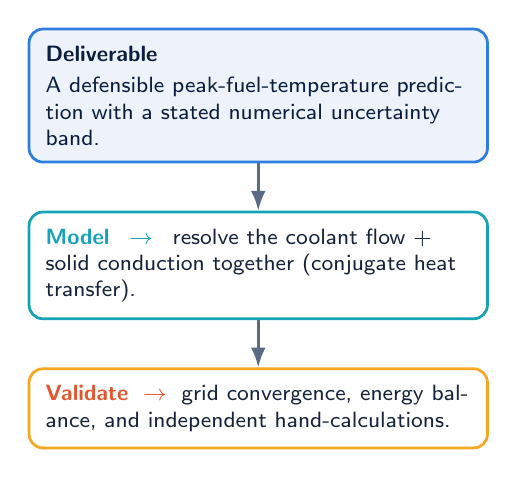
\begin{tikzpicture}[font=\footnotesize, node distance=6mm]
  \node[rounded corners=5pt, draw=RadBlue, line width=1pt, fill=RadPanel,
        text width=5.4cm, inner sep=6pt] (goal)
        {\bfseries\color{RadNavy} Deliverable\\[2pt]\normalfont A defensible peak-fuel-temperature prediction with a stated numerical uncertainty band.};
  \node[below=of goal, rounded corners=5pt, draw=RadTeal, line width=1pt,
        text width=5.4cm, inner sep=6pt] (m1)
        {\color{RadTeal}\bfseries Model $\;\to\;$ \normalfont\color{RadInk} resolve the coolant flow + solid conduction together (conjugate heat transfer).};
  \node[below=of m1, rounded corners=5pt, draw=RadAmber, line width=1pt,
        text width=5.4cm, inner sep=6pt] (m2)
        {\color{RadHot}\bfseries Validate $\;\to\;$ \normalfont\color{RadInk} grid convergence, energy balance, and independent hand-calculations.};
  \draw[-{Latex[length=2.5mm]},RadGray,line width=1pt] (goal)--(m1);
  \draw[-{Latex[length=2.5mm]},RadGray,line width=1pt] (m1)--(m2);
\end{tikzpicture}
\end{column}
\end{columns}
\end{frame}

%============================================================================
\sectiondivider{A}{ACTION}{Geometry, physics, solver --- and the mesh-quality problem that quietly moved the answer 87\,\textdegree C.}{03}

%----------------------------------------------------------------------------
\begin{frame}{Action 1 --- The unit-cell geometry}
\begin{columns}[T]
\begin{column}{0.45\textwidth}
\vspace{0.15cm}
\centering
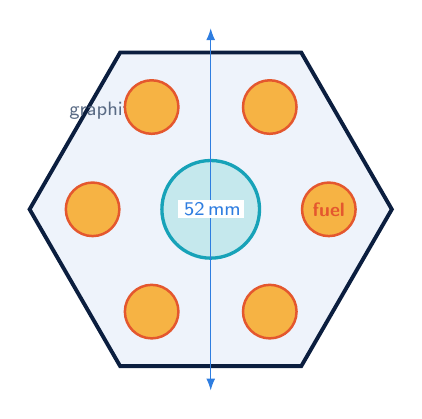
\begin{tikzpicture}[scale=1.0]
  % hexagon
  \node[regular polygon, regular polygon sides=6, draw=RadNavy, line width=1.4pt,
        fill=RadPanel, minimum size=4.6cm, rotate=0] (hex) at (0,0){};
  % graphite label
  \node[text=RadGray, font=\scriptsize] at (-1.35,1.25) {graphite};
  % coolant channel
  \fill[RadTeal!25, draw=RadTeal, line width=1.2pt] (0,0) circle (0.62);
  \node[text=RadTeal, font=\scriptsize\bfseries] at (0,0) {He};
  % fuel compacts on ring
  \foreach \a in {0,60,...,300}{
    \fill[RadAmber!85, draw=RadHot, line width=0.9pt] (\a:1.5) circle (0.34);
  }
  \node[text=RadHot, font=\scriptsize\bfseries] at (0:1.5) {fuel};
  % dims
  \draw[{Latex[length=1.5mm]}-{Latex[length=1.5mm]}, RadBlue] (90:2.3) -- (270:2.3)
        node[midway,fill=white,inner sep=1pt,text=RadBlue,font=\scriptsize]{$\varnothing$\,52\,mm};
\end{tikzpicture}\\[3pt]
{\color{RadGray}\scriptsize Cross-section (extruded 0.8\,m axially).}
\end{column}
\begin{column}{0.55\textwidth}
\vspace{0.1cm}
One hexagonal graphite prism, a central helium coolant channel, and a ring of six TRISO fuel compacts --- built parametrically in \kw{gmsh} (OpenCASCADE), fragmented so all regions share conforming faces, then extruded.
\vspace{0.2cm}

{\footnotesize
\begin{tabular}{@{}l r@{}}
\toprule
\rowcolor{RadPanel}\textbf{Parameter} & \textbf{Value}\\
\midrule
Hex circumradius & 30\,mm\\
Coolant channel dia. & 16\,mm\\
Fuel compact dia.\ ($\times$6) & 12.4\,mm\\
Fuel-compact ring radius & 18.8\,mm\\
Active height (axial) & 0.80\,m\\
\bottomrule
\end{tabular}}
\vspace{0.1cm}

{\color{RadGray}\footnotesize 3 volumes $\to$ cellZones via \texttt{gmshToFoam}.}
\end{column}
\end{columns}
\end{frame}

%----------------------------------------------------------------------------
\begin{frame}{Action 2 --- Physics \& solver setup}
\begin{columns}[T]
\begin{column}{0.54\textwidth}
\textbf{\color{RadNavy}Solver:} steady \kw{\texttt{chtMultiRegionFoam}} (OpenFOAM 7) --- conjugate heat transfer across a coupled thermal interface.
\vspace{0.15cm}
\begin{itemize}\small
  \item \kw{Two regions only:} \texttt{fluid} (helium, compressible ideal gas) and \texttt{solid} (graphite + fuel).
  \item \kw{Fuel} = a \texttt{topoSet} heat-source \texttt{cellZone} inside the solid, driven by \texttt{fvOptions} --- the standard way to embed a volumetric fission source and avoid a fragmented mesh.
  \item \kw{Turbulence:} $k$--$\varepsilon$ with wall functions (channel $Re\approx1.2\times10^{4}$, turbulent).
  \item \kw{Boundaries:} adiabatic outer wall + ends (symmetry); coupled fluid$\leftrightarrow$solid interface.
\end{itemize}
\end{column}
\begin{column}{0.46\textwidth}
\vspace{0.1cm}
\begin{block}{Operating point}
\small
\begin{tabular}{@{}l r@{}}
Helium pressure & 3\,MPa\\
Inlet temperature & 300\,\textdegree C\\
Bulk velocity & $\sim$10\,m/s\\
Reynolds number & $\sim$1.2$\times$10$^{4}$\\
Fuel power density $q'''$ & 7\,MW/m$^{3}$\\
\end{tabular}
\end{block}
\vspace{-0.1cm}
{\color{RadGray}\footnotesize \faCheckCircle\; Internal sanity checks passed on the first converged run: helium density \kw{2.52\,kg/m$^3$} and fuel$\to$wall conduction \kw{$\Delta T\approx11$\,\textdegree C} both matched hand-calcs.}
\end{column}
\end{columns}
\end{frame}

%----------------------------------------------------------------------------
\begin{frame}{Action 3 --- The mesh-quality problem (and the fix)}
\vspace{-0.1cm}
{\small The first mesh used \kw{triangular} prisms; triangles on the curved channel wall drove \amberkw{max non-orthogonality $\sim$86\textdegree}, degrading the conduction (Laplacian) term.}
\vspace{0.08cm}

\begin{columns}[T]
\begin{column}{0.6\textwidth}
{\footnotesize\renewcommand{\arraystretch}{1.12}
\begin{tabular}{@{}l c c c@{}}
\toprule
\rowcolor{RadPanel}\textbf{Metric} & \textbf{Tri-prism} & \textbf{Hex (fix)} & \textbf{Target}\\
\midrule
Cell type & 100\% prism & \textbf{100\% hex} & ---\\
Non-orth.\ max (fluid) & 86.0\textdegree & \textbf{15.2\textdegree} & $<$70\textdegree\\
Non-orth.\ avg (fluid) & 61.8\textdegree & \textbf{3.5\textdegree} & $<$30\textdegree\\
Non-orth.\ max (solid) & 86.0\textdegree & \textbf{36.9\textdegree} & $<$70\textdegree\\
Non-orth.\ avg (solid) & 57.6\textdegree & \textbf{10.1\textdegree} & $<$30\textdegree\\
\bottomrule
\end{tabular}}\\[3pt]
{\color{RadGray}\footnotesize Max skewness 0.26 $\to$ 0.66 (target $<$4); both regions stay a single connected mesh.}
\end{column}
\begin{column}{0.4\textwidth}
\vspace{-0.1cm}
\begin{block}{The fix (ADR-17)}
\small \kw{Recombine} to quads $\to$ extrude to \kw{hexahedra}, plus \kw{graded near-wall refinement} (targets $y^{+}\!\approx\!30$).
\end{block}
\vspace{-0.15cm}
{\color{RadGray}\footnotesize gmsh's structured BL field can't touch the conformal internal coolant wall; \texttt{snappyHexMesh addLayers} is the route to true inflation layers.}
\end{column}
\end{columns}
\vspace{-0.2cm}
\begin{center}
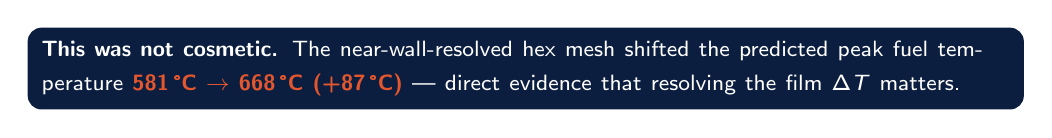
\begin{tikzpicture}
\node[rounded corners=5pt, fill=RadNavy, text=white, inner sep=5pt, text width=12.3cm]
{\footnotesize \textbf{This was not cosmetic.} The near-wall-resolved hex mesh shifted the predicted peak fuel temperature \amberkw{581\,\textdegree C $\to$ 668\,\textdegree C (+87\,\textdegree C)} --- direct evidence that resolving the film $\Delta T$ matters.};
\end{tikzpicture}
\end{center}
\end{frame}

%============================================================================
\sectiondivider{R}{RESULT}{A grid-independent peak fuel temperature --- corroborated three independent ways.}{04}

%----------------------------------------------------------------------------
\begin{frame}{Result 1 --- Peak fuel temperature}
\begin{columns}[T]
\begin{column}{0.5\textwidth}
\centering
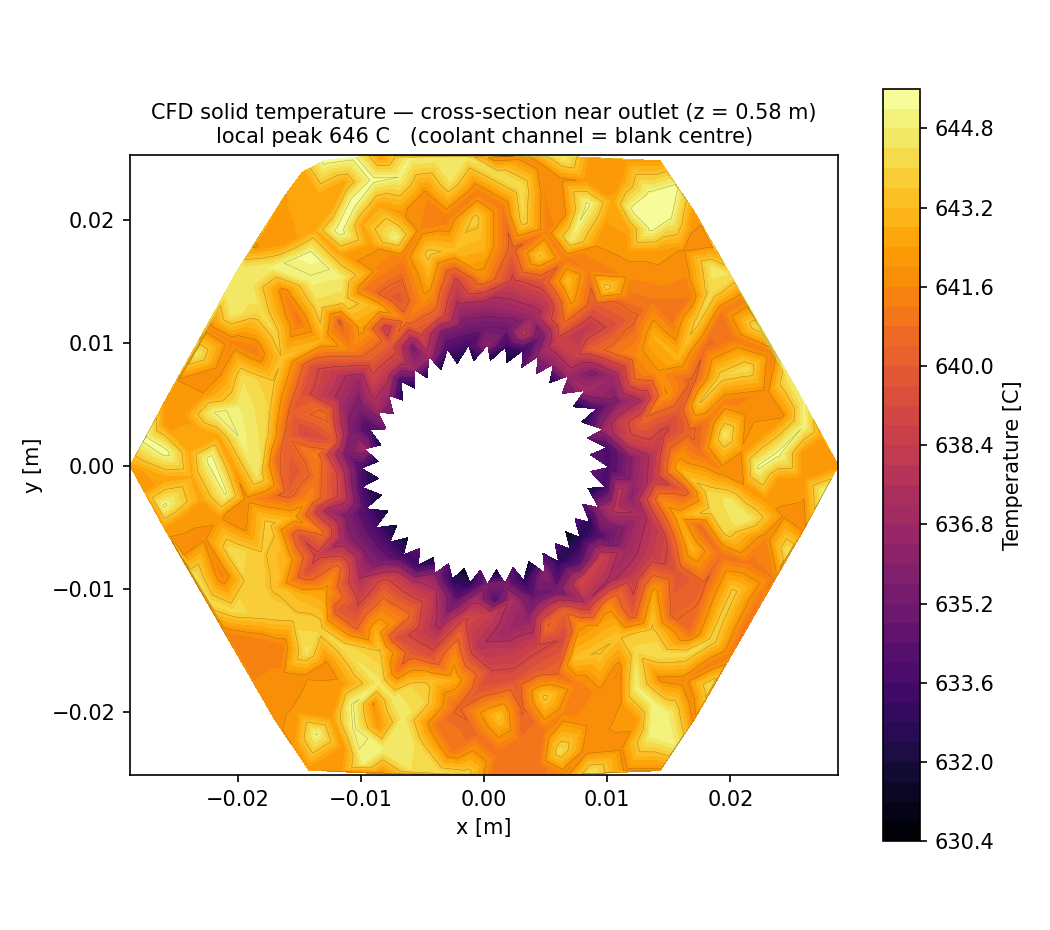
\includegraphics[height=4.05cm]{figures/cfd_cross_section.png}\\
{\color{RadGray}\scriptsize Solid temperature near outlet. Coolant channel = blank centre; hottest graphite sits between fuel compacts.}
\end{column}
\begin{column}{0.5\textwidth}
\centering
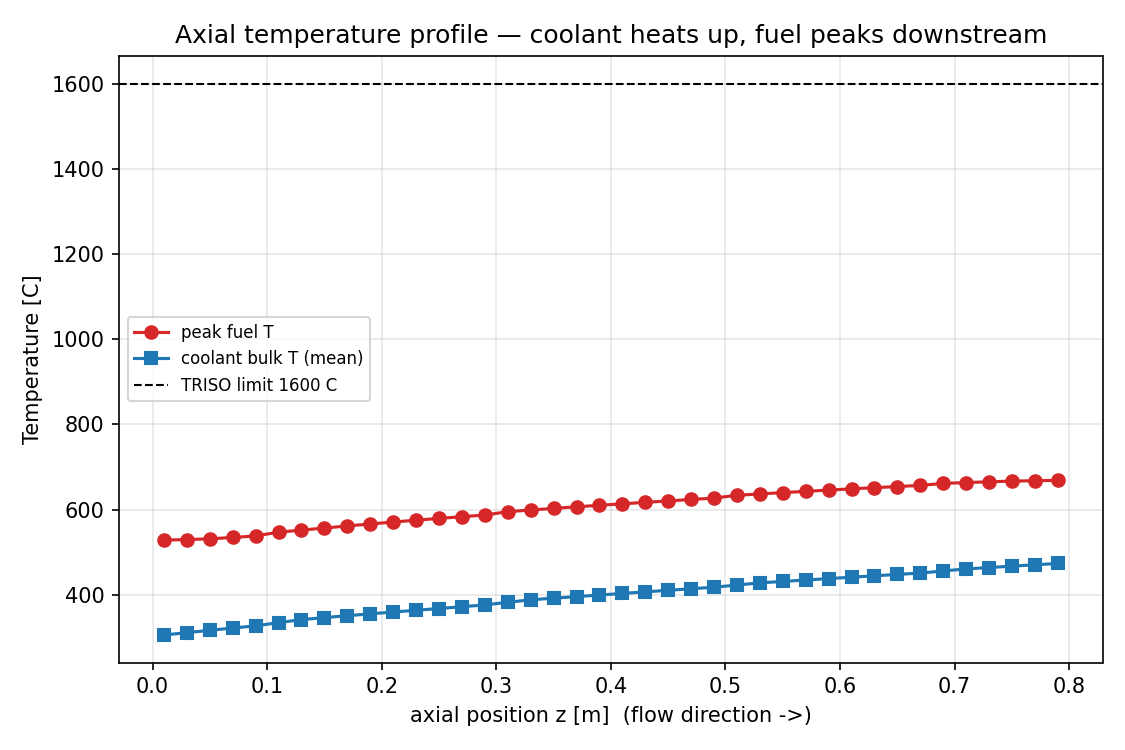
\includegraphics[height=4.05cm]{figures/cfd_axial_profile.png}\\
{\color{RadGray}\scriptsize Fuel peaks downstream as the coolant heats up; both stay far below the 1600\,\textdegree C limit.}
\end{column}
\end{columns}
\vspace{0.1cm}
\begin{center}

\begin{tikzpicture}
\node[rounded corners=6pt, fill=RadPanel2, draw=RadBlue, line width=1pt, inner sep=6pt, text width=11.8cm, align=center]
{\normalsize \textbf{\color{RadNavy}Peak fuel temperature $=$ \amberkw{670 $\pm$ 2\,\textdegree C}} \; --- \; $\sim$\textbf{930\,\textdegree C} margin to the 1600\,\textdegree C TRISO limit.};
\end{tikzpicture}
\end{center}
\end{frame}

%----------------------------------------------------------------------------
\begin{frame}{Result 2 --- Solution verification (grid convergence)}
\begin{columns}[T]
\begin{column}{0.52\textwidth}
\small A prediction needs a \kw{numerical uncertainty band}. I ran the normal case on three systematically refined hex meshes:
\vspace{0.15cm}

{\footnotesize
\begin{tabular}{@{}l c c@{}}
\toprule
\rowcolor{RadPanel}\textbf{Hex mesh} & \textbf{Cells} & \textbf{Peak fuel T}\\
\midrule
Coarse & 14.6k & 669.3\,\textdegree C\\
\rowcolor{RadPanel2}Medium (production) & 28.3k & 668.3\,\textdegree C\\
Fine & 56.5k & 672.0\,\textdegree C\\
\bottomrule
\end{tabular}}
\vspace{0.2cm}

\begin{itemize}\small
  \item Grid-independent to \amberkw{$\pm$2\,\textdegree C (0.56\%)} across a \kw{4$\times$} cell range.
  \item Convergence is oscillatory (numerical noise floor), so I report the oscillation amplitude as the uncertainty.
\end{itemize}
\end{column}
\begin{column}{0.48\textwidth}
\vspace{0.1cm}
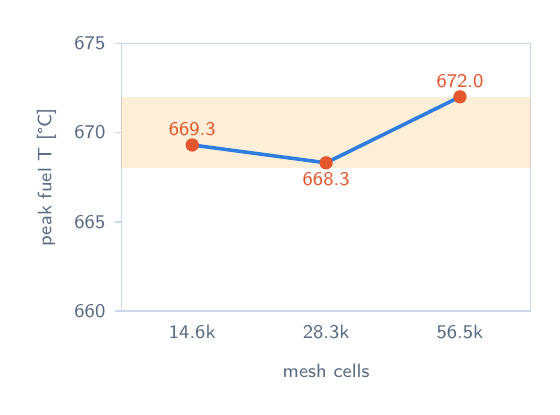
\begin{tikzpicture}[font=\scriptsize]
  \begin{scope}
  \def\W{5.2}\def\H{3.4}
  \draw[RadLine] (0,0) rectangle (\W,\H);
  % y ticks 660..675
  \foreach \y/\lab in {0.0/660,1.13/665,2.27/670,3.4/675}{
     \draw[RadLine] (0,\y)--(-0.08,\y); \node[left,text=RadGray] at (-0.08,\y){\lab};}
  \node[rotate=90, text=RadGray] at (-0.95,\H/2){peak fuel T [\textdegree C]};
  % x labels
  \foreach \x/\lab in {0.9/14.6k,2.6/28.3k,4.3/56.5k}{
     \node[below,text=RadGray] at (\x,-0.05){\lab};}
  \node[below,text=RadGray] at (\W/2,-0.55){mesh cells};
  % band 668-672 -> map T: y=(T-660)/15*H
  \fill[RadAmber,opacity=0.18] (0,{(668-660)/15*\H}) rectangle (\W,{(672-660)/15*\H});
  % points 669.3,668.3,672.0
  \coordinate (p1) at (0.9,{(669.3-660)/15*\H});
  \coordinate (p2) at (2.6,{(668.3-660)/15*\H});
  \coordinate (p3) at (4.3,{(672.0-660)/15*\H});
  \draw[RadBlue,line width=1.3pt] (p1)--(p2)--(p3);
  \foreach \p in {p1,p2,p3}{\fill[RadHot] (\p) circle (2.4pt);}
  \node[above,text=RadHot] at (p1){669.3};
  \node[below,text=RadHot] at (p2){668.3};
  \node[above,text=RadHot] at (p3){672.0};
  \end{scope}
\end{tikzpicture}\\[3pt]
{\color{RadGray}\footnotesize The 66\,\textdegree C gap vs.\ a coarse tri-prism (Richardson 604\,\textdegree C) is that mesh smearing the near-wall film $\Delta T$ --- the hex value is the trustworthy one.}
\end{column}
\end{columns}
\end{frame}

%----------------------------------------------------------------------------
\begin{frame}{Result 3 --- Validation (energy \& mass balance)}
\vspace{-0.05cm}
{\small On the converged solution, three \emph{independent} measures of the heat leaving the cell must agree if the physics is right. They close to \amberkw{0.01\%}.}
\vspace{0.25cm}

\begin{columns}[c]
\begin{column}{0.62\textwidth}
\centering
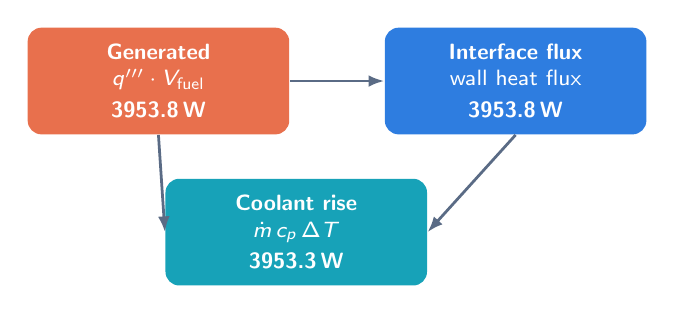
\begin{tikzpicture}[font=\footnotesize]
  \node[rounded corners=5pt, fill=RadHot!85, text=white, inner sep=6pt, text width=2.9cm, align=center] (gen)
    {\textbf{Generated}\\ $q'''\!\cdot\!V_\text{fuel}$\\[2pt] \bfseries 3953.8\,W};
  \node[rounded corners=5pt, fill=RadBlue, text=white, inner sep=6pt, text width=2.9cm, align=center, right=1.2cm of gen] (wall)
    {\textbf{Interface flux}\\ wall heat flux\\[2pt] \bfseries 3953.8\,W};
  \node[rounded corners=5pt, fill=RadTeal, text=white, inner sep=6pt, text width=2.9cm, align=center, below=0.55cm of gen, xshift=1.75cm] (cool)
    {\textbf{Coolant rise}\\ $\dot m\,c_p\,\Delta T$\\[2pt] \bfseries 3953.3\,W};
  \draw[-{Latex[length=2mm]},RadGray,line width=1pt] (gen)--(wall);
  \draw[-{Latex[length=2mm]},RadGray,line width=1pt] (gen.south)--(cool.west);
  \draw[-{Latex[length=2mm]},RadGray,line width=1pt] (wall.south)--(cool.east);
\end{tikzpicture}\\[4pt]
{\color{RadGray}\scriptsize Generated $=$ crosses the wall $=$ carried out by the coolant.}
\end{column}
\begin{column}{0.38\textwidth}
\begin{itemize}\small
  \item \kw{Mass} conserves to 0.000\% ($\dot m = 5.05$\,g/s, in $=$ out).
  \item Coolant bulk $\Delta T = 150.8$\,K (outlet 451\,\textdegree C) --- matches the $\sim$154\,K hand-calc.
  \item OpenFOAM function objects ($T_\text{out}=723.83$\,K, $\dot m=5.047$\,g/s) match the independent Python field parser exactly.
\end{itemize}
\end{column}
\end{columns}
\vspace{0.15cm}
{\color{RadGray}\footnotesize The adiabatic unit-cell symmetry makes this balance \emph{exact} by construction --- all generated heat has to leave through the coolant, so closure to 0.01\% is a strong correctness check.}
\end{frame}

%----------------------------------------------------------------------------
\begin{frame}{Result --- The headline, in four numbers}
\vspace{0.5cm}
\begin{columns}[c]
\begin{column}{0.25\textwidth}\centering
\stattile{RadHot}{670}{\textdegree C}{peak fuel T ($\pm$2\textdegree C)}
\end{column}
\begin{column}{0.25\textwidth}\centering
\stattile{RadAmber}{$\sim$930}{\textdegree C}{margin to TRISO limit}
\end{column}
\begin{column}{0.25\textwidth}\centering
\stattile{RadBlue}{0.01}{\%}{energy-balance closure}
\end{column}
\begin{column}{0.25\textwidth}\centering
\stattile{RadTeal}{0.56}{\%}{grid-independence band}
\end{column}
\end{columns}
\vspace{0.7cm}
\begin{center}
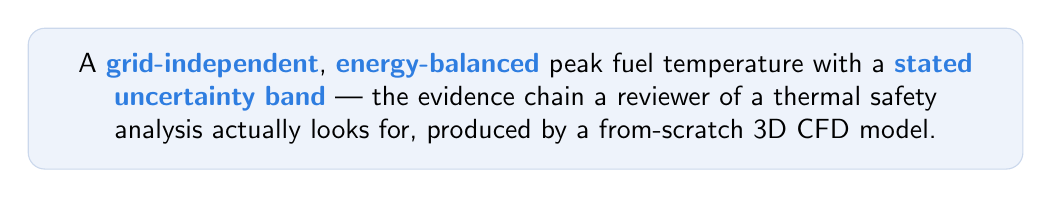
\begin{tikzpicture}
\node[rounded corners=6pt, fill=RadPanel, draw=RadLine, inner sep=9pt, text width=12cm, align=center]
{\normalsize A \kw{grid-independent}, \kw{energy-balanced} peak fuel temperature with a \kw{stated uncertainty band} --- the evidence chain a reviewer of a thermal safety analysis actually looks for, produced by a from-scratch 3D CFD model.};
\end{tikzpicture}
\end{center}
\end{frame}

%----------------------------------------------------------------------------
\begin{frame}{Scope, limitations \& next steps}
\begin{columns}[T]
\begin{column}{0.5\textwidth}
\textbf{\color{RadNavy}\faBalanceScale\; Honest limitations}
\begin{itemize}\small
  \item Unit-cell \kw{symmetry} $\Rightarrow$ adiabatic outer walls; block-edge and inter-cell effects not resolved.
  \item $y^{+}\!\approx\!19$ sits in the buffer/log range --- slightly below the ideal wall-function band; aspect ratio 28--37 from long axial cells.
  \item No fully structured inflation layer (gmsh limitation); graded refinement captures most of the benefit.
  \item Steady state --- absolute values are indicative given representative (non-vendor) material data.
\end{itemize}
\end{column}
\begin{column}{0.5\textwidth}
\textbf{\color{RadNavy}\faArrowRight\; Natural next steps}
\begin{itemize}\small
  \item \kw{\texttt{snappyHexMesh addLayers}} for true wall-normal inflation layers and a cleaner $y^{+}$.
  \item \kw{FEM$\leftrightarrow$CFD cross-check}: compare against my 2D finite-element conduction solver (element vs.\ volume, wall-$h$ vs.\ resolved flow).
  \item \kw{Loss-of-forced-cooling} case in 3D + a \kw{transient} run with an ANS-5.1 decay-heat curve --- the walk-away-safe story, time-accurate.
\end{itemize}
\vspace{0.2cm}
{\color{RadGray}\footnotesize Every limitation above is stated, bounded, and has a defined path to close it.}
\end{column}
\end{columns}
\end{frame}

%----------------------------------------------------------------------------
%  CLOSING
%----------------------------------------------------------------------------
\begin{frame}[plain]
\begin{tikzpicture}[remember picture,overlay]
  \fill[RadNavy] (current page.south west) rectangle (current page.north east);
  \shade[bottom color=RadBlue, top color=RadHot]
     ([xshift=1.25cm,yshift=-1.75cm]current page.north west) rectangle ([xshift=1.42cm,yshift=-0.45cm]current page.north west);
  \node[anchor=north west, text=RadAmber, font=\bfseries] at ([xshift=1.75cm,yshift=-0.75cm]current page.north west){THANK YOU};
  \node[anchor=north west] at ([xshift=1.7cm,yshift=-2.35cm]current page.north west)
     {\begin{minipage}{12.7cm}\color{white}\fontsize{18}{23}\selectfont\bfseries
       A validated 3D peak-fuel-temperature prediction --- and the reasoning behind every number.\end{minipage}};
  % recap chips
  \node[anchor=north west] at ([xshift=1.72cm,yshift=-5.25cm]current page.north west)
    {\begin{minipage}{12.7cm}\color{RadBlueL}\small
      \ding{110}\; unit-cell \texttt{chtMultiRegionFoam} \qquad
      \ding{110}\; hex mesh fix (+87\,\textdegree C) \\[4pt]
      \ding{51}\; 670\,$\pm$\,2\,\textdegree C peak \quad 0.01\% energy closure \quad grid-independent
    \end{minipage}};
  \fill[RadNavy2] (current page.south west) rectangle ([yshift=1.15cm]current page.south east);
  \node[anchor=west, text=white] at ([xshift=1.7cm,yshift=0.57cm]current page.south west)
     {\footnotesize\bfseries Samay Shah \quad\textbullet\quad {\color{RadBlueL}\mdseries 3D CFD Conjugate Heat-Transfer Study}};
  \node[anchor=east, text=RadAmber] at ([xshift=-1.4cm,yshift=0.57cm]current page.south east){\footnotesize\bfseries Questions welcome};
\end{tikzpicture}
\end{frame}

\end{document}
